\section{Auswertung}

In der folgenden Auswertung werden zuerst die beiden Relaxationszeiten $T\ua{1}$
sowie $T\ua{2}$ bestimmt. Mithilfe von kann dann die Diffusionskonstante $D$ sowie
der Molekülradius bestimmt werden. Der Molekülradius wird am Ende zudem mit
den Radien verglichen, die sich aus dem Molekulargewicht und dem Van-der-Waals-Kovolumen
ergeben.

\subsection{Bestimmung der longitudinalen Relaxationszeit $T\ua{1}$}

Die aufgenommenen Daten für die Bestimmung von $T\ua{1}$ sind Tabelle \ref{tab:T1}
eingetragen sowie in Abbildung \ref{fig:T1} grafisch dargestellt.

\begin{table}
  \centering
  \caption{Messdaten für die Spannungamplituden des ersten Echos bei verschiedenen
  Pulsabständen.}
  \label{tab:T1}
  \begin{tabular}{S  S | S  S}
    \toprule
    {$\tau / \si{ms}$} & {$U / \si{mV}$} & {$\tau /\si{ms}$} & {$U / \si{mV}$} \\
    \midrule
    1  & -785 & 100  & -633 \\
    2  & -780 & 200  & -565   \\
    3  & -765 & 500  & -395   \\
    5  & -745 & 1000 & -195   \\
    8  & -745 & 1500 &   35   \\
    9  & -735 & 2000 &  118   \\
    13 & -730 & 4000 &  612   \\
    20 & -715 & 7000 &  643 \\
    50 & -665 & 9000 &  700   \\
    75 & -648 & &           \\
    \bottomrule
  \end{tabular}
\end{table}


Um $T1$ zu bestimmen werden die experimentellen Daten an eine Exponentialfunktion
der folgenden Form gefittet:

\begin{equation}
  M(t) = M\ua{0}(1-2\exp{(-\frac{t}{T_1})})+M\ua{1}.
\end{equation}

Für die verschiedenen Parameter ergeben sich damit folgende Werte:
\begin{align}
  M\ua{0} &= (0.73\pm0.02)\,\si{V} \\
  M\ua{1} &= (0.04\pm0.03)\,\si{V} \\
  T\ua{1} &= (1.54\pm0.12)\,\si{s}
\end{align}

\begin{figure}
  \centering
  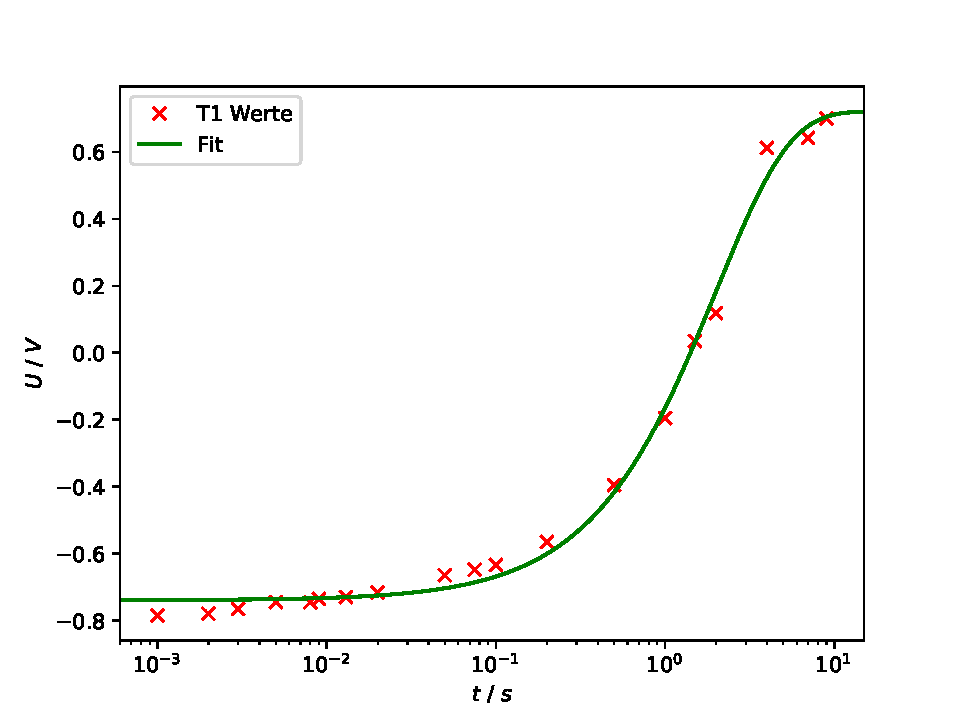
\includegraphics[width=\textwidth]{Plots2/T1.pdf}
  \caption{Gemessene Signalhöhe des Echos gegen den zeitlichen Abstand der beiden Pulse.}
  \label{fig:T1}
\end{figure}

\subsection{Bestimmung der transversalen Relaxationszeit $T\ua{2}$}

Um die transversale Relaxationszeit $T\ua{2}$ zu bestimmen wird das Meiboom-Gill Verfahren
verwendet. Zudem ist in Abbildung \ref{fig:T2CP} einmal die Burstsequenz mit dem
Carr-Purcell-Verfahren dargestellt.

\begin{figure}\centering
  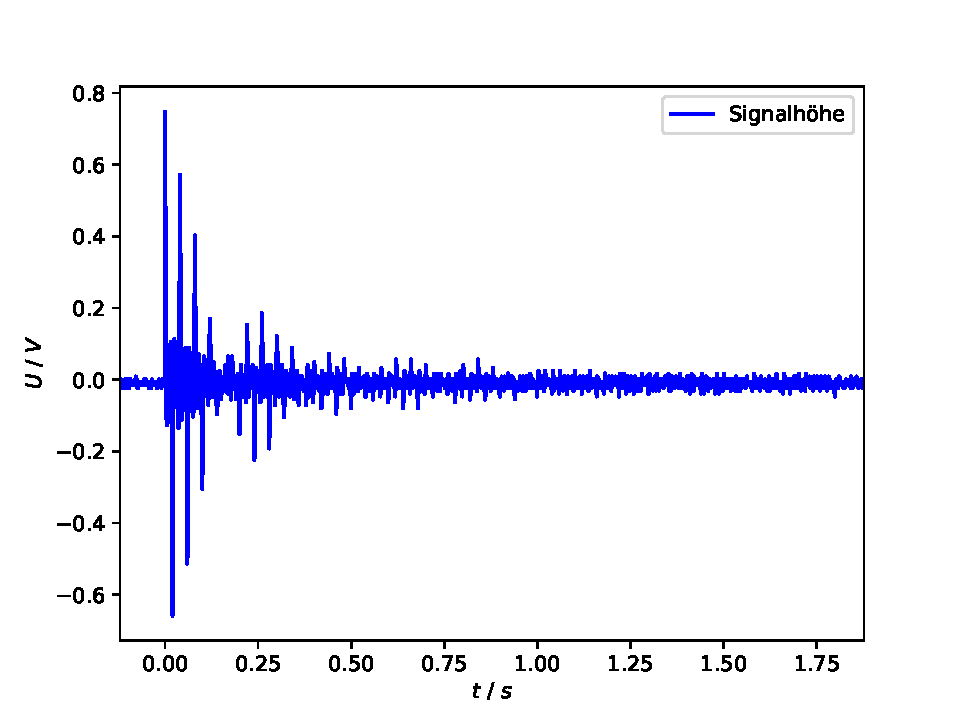
\includegraphics[width=\textwidth]{Plots2/T2CP.pdf}
  \caption{Signale der transversalen Magnetisierung mit der Carr-Purcell-Methode
  bei einem Pulsabstan von $\tau = \SI{2}{ms}$. }
  \label{fig:T2CP}
\end{figure}

In Abbildung \ref{fig:T2} ist die Burstsequenz mit der Meiboom-Gill Methode
dargestellt. Die verwendeten 
